\documentclass[tikz,border=4pt]{standalone}
\usepackage{tikz}
\usepackage{amsmath}
\usetikzlibrary{matrix,positioning}

\begin{document}
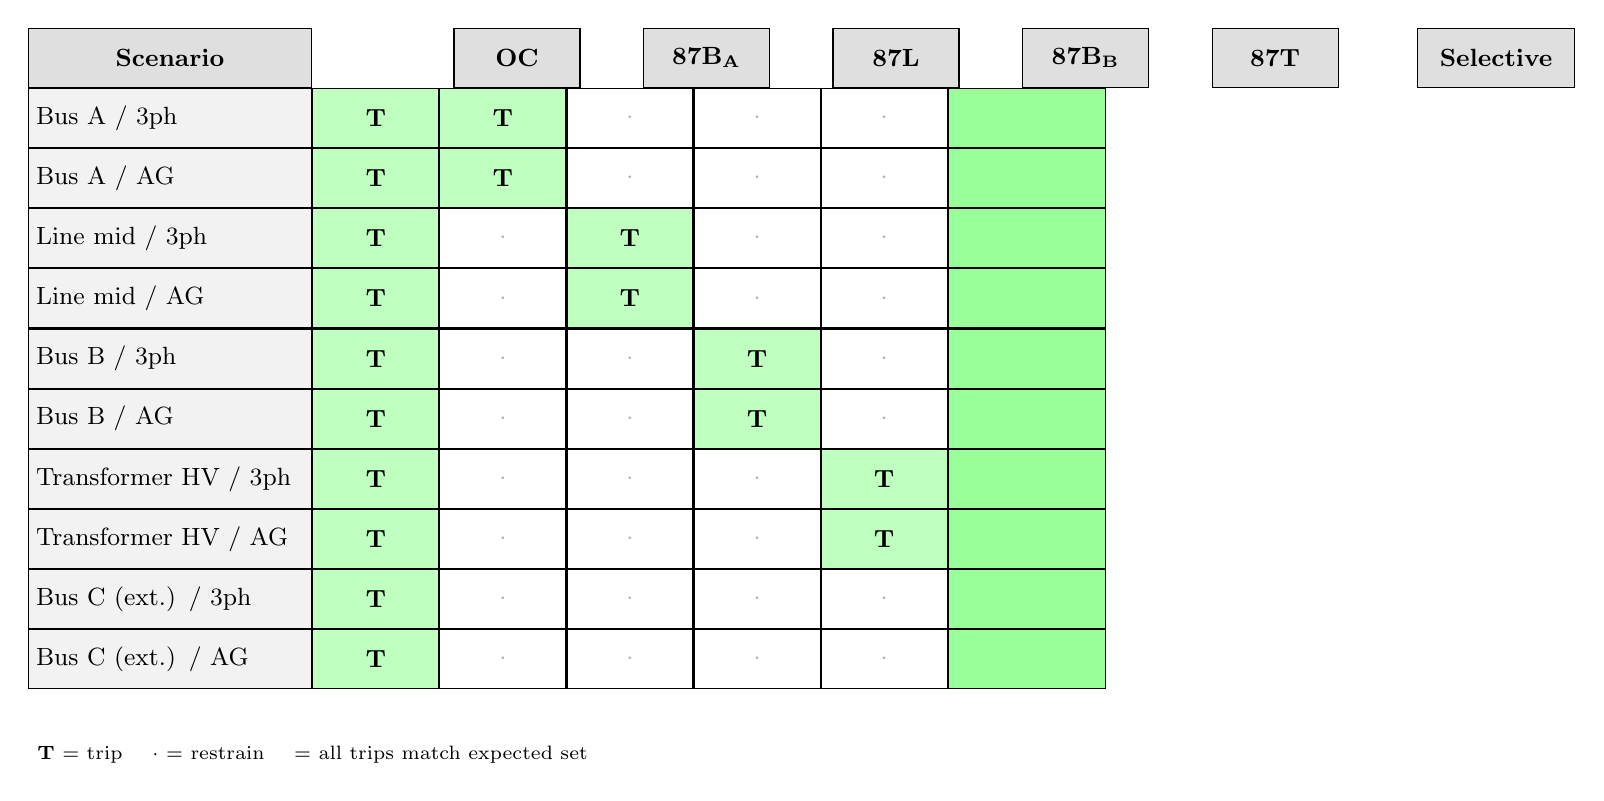
\begin{tikzpicture}[
    cell/.style={draw,minimum width=1.6cm,minimum height=0.75cm,
                 font=\small,align=center,inner sep=0pt},
    hdr/.style={cell,fill=gray!25,font=\small\bfseries},
    trip/.style={cell,fill=green!25,font=\small\bfseries},
    rest/.style={cell,fill=white,font=\small,text=gray!60},
    scen/.style={cell,fill=gray!10,font=\small,align=left,
                 minimum width=3.6cm,text width=3.4cm},
]

% ---- Column headers -------------------------------------------------
\def\col#1#2{\node[hdr,xshift={#1*1.6cm}] {#2};}

\node[hdr,minimum width=3.6cm] (h0) at (0,0) {Scenario};
\node[hdr,xshift=2.6cm]  (h1) at (h0.east) {OC};
\node[hdr,xshift=1.6cm]  (h2) at (h1.east) {87B\textsubscript{A}};
\node[hdr,xshift=1.6cm]  (h3) at (h2.east) {87L};
\node[hdr,xshift=1.6cm]  (h4) at (h3.east) {87B\textsubscript{B}};
\node[hdr,xshift=1.6cm]  (h5) at (h4.east) {87T};
\node[hdr,xshift=2.0cm,minimum width=2.0cm]  (h6) at (h5.east) {Selective};

% Each row: fault scenario, then T/· for each relay
\def\row#1#2#3#4#5#6#7#8{%
    \node[scen,yshift={-#1*0.75cm},below=0pt of h0.south west,anchor=north west]
         (r#1s) {#2};
    \node[#3,right=0pt of r#1s] (r#1a) {#4};
    \node[#3,right=0pt of r#1a] (r#1b) {#5};
    \node[#3,right=0pt of r#1b] (r#1c) {#6};
    \node[#3,right=0pt of r#1c] (r#1d) {#7};
    \node[#3,right=0pt of r#1d] (r#1e) {#8};
}

% row: index, label, cell-style, OC, 87B_A, 87L, 87B_B, 87T  (+ selective auto)

% row 1: bus_A / 3ph
\node[scen,below=0pt of h0.south west,anchor=north west]
     (r1s) {Bus A / 3ph};
\node[trip,right=0pt of r1s]   (r1a) {\textbf{T}};
\node[trip,right=0pt of r1a]   (r1b) {\textbf{T}};
\node[rest,right=0pt of r1b]   (r1c) {$\cdot$};
\node[rest,right=0pt of r1c]   (r1d) {$\cdot$};
\node[rest,right=0pt of r1d]   (r1e) {$\cdot$};
\node[cell,fill=green!40,right=0pt of r1e,minimum width=2.0cm] {\checkmark};

% row 2: bus_A / ag
\node[scen,below=0pt of r1s.south west,anchor=north west]
     (r2s) {Bus A / AG};
\node[trip,right=0pt of r2s]   (r2a) {\textbf{T}};
\node[trip,right=0pt of r2a]   (r2b) {\textbf{T}};
\node[rest,right=0pt of r2b]   (r2c) {$\cdot$};
\node[rest,right=0pt of r2c]   (r2d) {$\cdot$};
\node[rest,right=0pt of r2d]   (r2e) {$\cdot$};
\node[cell,fill=green!40,right=0pt of r2e,minimum width=2.0cm] {\checkmark};

% row 3: line_mid / 3ph
\node[scen,below=0pt of r2s.south west,anchor=north west]
     (r3s) {Line mid / 3ph};
\node[trip,right=0pt of r3s]   (r3a) {\textbf{T}};
\node[rest,right=0pt of r3a]   (r3b) {$\cdot$};
\node[trip,right=0pt of r3b]   (r3c) {\textbf{T}};
\node[rest,right=0pt of r3c]   (r3d) {$\cdot$};
\node[rest,right=0pt of r3d]   (r3e) {$\cdot$};
\node[cell,fill=green!40,right=0pt of r3e,minimum width=2.0cm] {\checkmark};

% row 4: line_mid / ag
\node[scen,below=0pt of r3s.south west,anchor=north west]
     (r4s) {Line mid / AG};
\node[trip,right=0pt of r4s]   (r4a) {\textbf{T}};
\node[rest,right=0pt of r4a]   (r4b) {$\cdot$};
\node[trip,right=0pt of r4b]   (r4c) {\textbf{T}};
\node[rest,right=0pt of r4c]   (r4d) {$\cdot$};
\node[rest,right=0pt of r4d]   (r4e) {$\cdot$};
\node[cell,fill=green!40,right=0pt of r4e,minimum width=2.0cm] {\checkmark};

% row 5: bus_B / 3ph
\node[scen,below=0pt of r4s.south west,anchor=north west]
     (r5s) {Bus B / 3ph};
\node[trip,right=0pt of r5s]   (r5a) {\textbf{T}};
\node[rest,right=0pt of r5a]   (r5b) {$\cdot$};
\node[rest,right=0pt of r5b]   (r5c) {$\cdot$};
\node[trip,right=0pt of r5c]   (r5d) {\textbf{T}};
\node[rest,right=0pt of r5d]   (r5e) {$\cdot$};
\node[cell,fill=green!40,right=0pt of r5e,minimum width=2.0cm] {\checkmark};

% row 6: bus_B / ag
\node[scen,below=0pt of r5s.south west,anchor=north west]
     (r6s) {Bus B / AG};
\node[trip,right=0pt of r6s]   (r6a) {\textbf{T}};
\node[rest,right=0pt of r6a]   (r6b) {$\cdot$};
\node[rest,right=0pt of r6b]   (r6c) {$\cdot$};
\node[trip,right=0pt of r6c]   (r6d) {\textbf{T}};
\node[rest,right=0pt of r6d]   (r6e) {$\cdot$};
\node[cell,fill=green!40,right=0pt of r6e,minimum width=2.0cm] {\checkmark};

% row 7: transformer_hv / 3ph
\node[scen,below=0pt of r6s.south west,anchor=north west]
     (r7s) {Transformer HV / 3ph};
\node[trip,right=0pt of r7s]   (r7a) {\textbf{T}};
\node[rest,right=0pt of r7a]   (r7b) {$\cdot$};
\node[rest,right=0pt of r7b]   (r7c) {$\cdot$};
\node[rest,right=0pt of r7c]   (r7d) {$\cdot$};
\node[trip,right=0pt of r7d]   (r7e) {\textbf{T}};
\node[cell,fill=green!40,right=0pt of r7e,minimum width=2.0cm] {\checkmark};

% row 8: transformer_hv / ag
\node[scen,below=0pt of r7s.south west,anchor=north west]
     (r8s) {Transformer HV / AG};
\node[trip,right=0pt of r8s]   (r8a) {\textbf{T}};
\node[rest,right=0pt of r8a]   (r8b) {$\cdot$};
\node[rest,right=0pt of r8b]   (r8c) {$\cdot$};
\node[rest,right=0pt of r8c]   (r8d) {$\cdot$};
\node[trip,right=0pt of r8d]   (r8e) {\textbf{T}};
\node[cell,fill=green!40,right=0pt of r8e,minimum width=2.0cm] {\checkmark};

% row 9: bus_C_load / 3ph
\node[scen,below=0pt of r8s.south west,anchor=north west]
     (r9s) {Bus C (ext.) / 3ph};
\node[trip,right=0pt of r9s]   (r9a) {\textbf{T}};
\node[rest,right=0pt of r9a]   (r9b) {$\cdot$};
\node[rest,right=0pt of r9b]   (r9c) {$\cdot$};
\node[rest,right=0pt of r9c]   (r9d) {$\cdot$};
\node[rest,right=0pt of r9d]   (r9e) {$\cdot$};
\node[cell,fill=green!40,right=0pt of r9e,minimum width=2.0cm] {\checkmark};

% row 10: bus_C_load / ag
\node[scen,below=0pt of r9s.south west,anchor=north west]
     (r10s) {Bus C (ext.) / AG};
\node[trip,right=0pt of r10s]  (r10a) {\textbf{T}};
\node[rest,right=0pt of r10a]  (r10b) {$\cdot$};
\node[rest,right=0pt of r10b]  (r10c) {$\cdot$};
\node[rest,right=0pt of r10c]  (r10d) {$\cdot$};
\node[rest,right=0pt of r10d]  (r10e) {$\cdot$};
\node[cell,fill=green!40,right=0pt of r10e,minimum width=2.0cm] {\checkmark};

% ---- Legend -------------------------------------------------------------
\node[font=\scriptsize,below=0.6cm of r10s.south west,anchor=north west]
    {\textbf{T} = trip \quad $\cdot$ = restrain \quad
     \checkmark = all trips match expected set};

\end{tikzpicture}
\end{document}
